\chapter{Fonctionnement général}
\section{Explication et justification de l'infrastructure}
\subsection{Général}
Nous disposons de deux machines pour mettre en place l'infrastructure.
Cela limite les choix d'architectures possible. Nous nous sommes tourné vers une 
architecture avec un serveur de centralisation des logs/flux, et un serveur 
d'indexation et d'exploitation de ces \gls{logs}. C'est une configuration assez standard
lorsque l'on met en place une pile ELK.

Cette configuration présente l'avantage de répartir la charge de travail de manière 
assez satisfaisante.Les deux points \textit{chauds} étant la réception des logs 
(~20-30 millions de lignes par jours) et le traitement de ces logs \textit{nettoyés}.


\begin{figure}[H]
\center
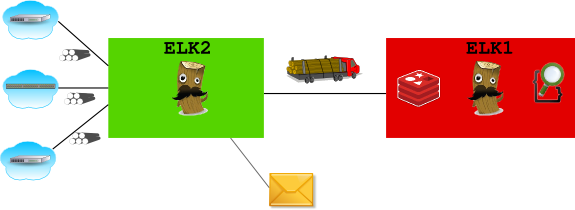
\includegraphics[width=1\textwidth]{stacksimple.png}
\label{fig:elkstack1}
\caption{Notre pile ELK}
\end{figure}

Il est encore possible en cas de besoin de répartir un peu mieux la charge
en déportant Kibana sur ELK2. Cependant son empreinte mémoire n'est pas très élevée
et ses besoins en processeur assez ponctuels, ce n'est donc pas un vrai problème.\\[5mm]

Il est possible de faire fonctionner logstash en temps qu'agent, soit en l'installant
directement sur un materiel, soit en le compilant spécifiquement pour un materiel.

Cela n'a pas été nécessaire puisque l'infrastructure réseau de Lorraine disposait 
déjà un système complètement fonctionnel sur syslog-ng\footnote{un système d'agent 
assez avancé permettant la centralisation de log}. 
Depuis très récemment (encore en beta à l'écriture de ces lignes) syslog-ng est 
capable d'envoyer ses logs vers Elasticsearch, cependant la version de syslog-ng
installée sur les équipements ne permet actuellement pas de le faire.

Sans entrer dans les détails, cette solutions n'aurait de toute façon pas été retenu,
car elle impliquait de centraliser et traiter les logs sur la même machine. Ce qui
aurait probablement eu des effets dramatiques sur les performances, ne parlons pas 
de la résilience.

Des informations concernant les infrastructures ont été distillées au long des différents
chapitres, vous trouverez en annexe la \hyperref[]{configuration de logstash elk2},
la configuration pour \hyperref[]{Logstash elk1}, le mapping des index \hyperref[]{d'état} et 
de \hyperref[]{firewall}. 

\subsubsection{Redis}
Nous nous servons de Redis comme d'un tampon (buffer), Logstash d'Elk2 envoie ses 
données vers Redis situé sur Elk1. Ces données sont ensuite récupérées sur par Logstash
d'Elk1 qui les envoie sur Elasticsearch.

L'intérêt d'avoir un Redis (et donc un Logstash) entre le Logstash Elk2 et Elasticsearch
est de fluidifier le trafic. Si Elasticsearch ne pouvait pas traiter immédiatement 
les données qui lui sont envoyés \footnote{cela arrive, latence disque dur, occupation
intensive du processeur, à cause d'une recherche Kibana\ldots} la file d'attente 
de Logstash serait immédiatement encombrée et donc de prévenir la perte données.

Sa configuration (\textbf{très simple}) est disponible en annexes.

\subsection{Analyse des performances}
Globalement en fin de stage, l'infrastructure ELK fonctionne comme demandé pour ses besoins.
Cependant, la marge de manoeuvre n'est pas très importante.

Concernant Elk2, la machine qui centralise les logs, pas de problèmesi. Nous pourrions
ajouter plus de trafic et ou faire un tri plus drastique (consommateur en CPU), il
y a de la marge. La ressource la plus exploité est le réseau, et la aussi il y a 
de la marge.





\section{Évolutions possible}
\subsection{Monitoring}
\subsection{Sécurité}
\subsection{Clusters}
